\begin{center}
  \textsf{Листок 2.}
\end{center}
\vspace{0.01mm}
\nopagebreak[2]
\task{ Тело начинает движение из точки $А$ и движется сначала
  равноускоренно в течении времени $t_0$, а затем с тем же по модулю
  ускорением равнозамедленно. Через какое время от начала движения
  тело вернётся в точку $А$?}

\task{ Время отправления электрички по расписанию 12:00. На ваших
  часах 12:00, но мимо вас уже начинает проезжать последний вагон,
  который движется мимо вас в течении 10 с. Последний вагон проходит
  мимо вас за 8 с. Электричка отправилась вовремя, и движется
  равноускоренно. На какое время отстают ваши часы? }

\taskpic{ Из миномёта ведут стрельбу по объектам, расположенным на склоне
  горы. На каком расстоянии от миномёта будут падать мины, если их
  начальная скорость $V$, угол наклона горы $\alpha$ и угол стрельбы по
  отношению к горизонту $\beta$?}{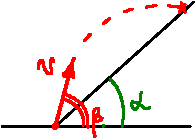
\includegraphics[width=4cm]{p09_7.pdf}}

\taskpic{ Утка летит по горизонтальной прямой с постоянной скоростью $U$. В
  неё бросил камень неопытный охотник, причём в момент броска
  скорость камня $V$ была направлена как раз на утку под углом $\alpha$ к
  горизонту. На какой высоте летела утка, если камень всё же попал в
  неё? }{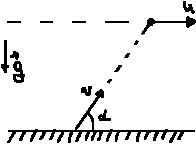
\includegraphics[width=4cm]{p09_8.pdf}}
